\chapter{Performance-Analyse der derzeitigen Implementierung}

\section{Komplexität}

\subsection{Speckle-Tracking}

Der erste Schritt des Speckle-Trackings ist die Feststellung der starren Verschiebung. Werden hierfür feste Werte angenommen, ist diese Komplexität konstant. Wird allerdings ein Korrelationsverfahren verwendet, so ist die Komplexität $\mathcal{O}\left(\glssymbol{resolution} \cdot log\left(\glssymbol{resolution}\right)\right)$ für die \gls{resolution}, da hierfür \glspl{FFT} eingesetzt werden. 

Der nächste Verarbeitungsschritt ist der erste Durchlauf. Hier werden die Eingabebilder zunächst durch die Selektion der \gls{ROI}, also auf die \glsfirst{rroi} \glssymbol{rroi} verkleinert und anschließend in Blöcke mit konstanter Größe aufgeteilt, welche dann ineinander mittels des Template-Matchings gesucht werden. Die Komplexität der einzelnen Suchvorgänge kann somit auch als konstant angesehen werden. Der Durchlauf braucht demzufolge $\mathcal{O}\left(\gls{rroi}\right)$ Schritte. Die anschließende Interpolation wird auf alle Pixel des Bildes angewandt und hat demzufolge eine Komplexität von $\mathcal{O}\left(\gls{rroi}\right)$.

Der zweite Durchlauf, der als nächstes folgt, werden Subbilder, wie \ref{sec:speckle-tracking} beschrieben, generiert. durch die \glsfirst{uap} \glssymbol{uap} wird \gls{rroi}, und damit auch die Komplexität dieses Teils, mit dem Faktor $\gls{uap}^2$ verringert. Die \glsfirst{corrsize} \glssymbol{corrsize} legt nimmt auf das Template-Matching Einfluss, dessen Komplexität nun bei $\mathcal{O}\left(\gls{corrsize} \cdot log\left(\gls{corrsize}\right)\right)$ liegt. Der Einfluss der \glsfirst{gridResol} \glssymbol{gridResol} ist, ähnlich zu \gls{uap}, eine Verringerung mit dem Faktor $\gls{gridResol}^2$. Die Gesamtkomplexität der Template-Matchings im zweiten Durchlauf liegt somit bei:

\begin{center}
	$\mathcal{O}\left(\frac{\gls{rroi} \cdot \gls{corrsize} \cdot log\left(\gls{corrsize}\right)}{\left(\gls{uap}^2 \cdot \gls{gridResol}\right)^2}\right)$
\end{center}

Für die auf den Template-Matching-Prozess folgende Subpixel-Interpolierung werden neun Pixel in der Umgebung des Maximums jedes Übereinstimmungsmatrix interpoliert, womit dieser Schritt folgende Komplexität aufweist:

\begin{center}
	$\mathcal{O}\left(\frac{\gls{rroi}}{\left(\gls{uap}^2 \cdot \gls{gridResol}^2\right)}\right)$
\end{center}

Am Ende des Speckle-Tracking-Algorithmus wird versucht, nicht zuordenbare Ergebnisse mit einer anderen \glsfirst{corrsize} \glssymbol{corrsize} erneut zuzuordnen. Im schlimmsten Fall wird der zweite Durchlauf für die Hälfte der Subbilder \gls{ncorr}-fach wiederholt, wobei \gls{ncorr} die \glsdesc{ncorr} repräsentiert. Bei höheren Fehlerraten über 50\% bricht das Programm. In der hier als Grundlage vorliegenden Implementierung ist $\gls{ncorr} = 6$.

Die Gesamtkomplexität des Speckle-Tracking-Algorithmus liegt damit in der Komplexitätsklasse:

\begin{center}
	$\mathcal{O}\left(\frac{\gls{rroi} \cdot \gls{corrsize} \cdot log\left(\gls{corrsize}\right)}{\left(\gls{uap}^2 \cdot \gls{gridResol}\right)^2}\right)$
\end{center}

\subsection{Integration der Gradienten}

Um eine effiziente Integration der Gradienten zu ermöglichen, beruht der von \citeauthor{FC88} vorgeschlagene Algorithmus auf der Integration im Frequenzraum. Hierzu werden zuerst die Gradientenbilder mittels \glspl{FFT} in diesen Raum transformiert, dort in linearer Komplexität integriert und zum Schluss wieder zurück transformiert. 
Aufgrund der Verwendung von \glspl{FFT} befindet sich dieser Algorithmus in der Komplexitätsklasse:

\begin{center}
	$\mathcal{O}\left(\gls{resolution} \cdot log\left(\gls{resolution}\right)\right)$
\end{center}

\subsection{Hauptroutine}

Die Hauptroutine beginnt mit einer trivialen Parameterinitialisierung, die als linear angenommen werden kann. Auf diese folgt die Hauptschleife, welche für die \gls{N_Paare} jeweils ein mal ausgeführt wird. Hierzu werden zuerst die Sensorbilder mittels der bei der Kalibrierung ermittelten Werte mit einer Komplexität von $\mathcal{O}\left(\gls{resolution}\right)$ korrigiert. Dies wird gefolgt vom Speckle-Tracking-Algorithmus und der Integration der Gradienten. Die höchste Komplexität hat hier der Template-Matching-Algorithmus, welcher damit die Komplexitätsklasse und somit auch der gesamten Hauptroutine festlegt auf:

\begin{center}
	$\mathcal{O}\left(\frac{\gls{N_Paare} \cdot\gls{rroi} \cdot \gls{corrsize} \cdot log\left(\gls{corrsize}\right)}{\left(\gls{uap}^2 \cdot \gls{gridResol}\right)^2}\right)$
\end{center}

Dies liegt insbesondere für kleine \gls{uap} und \gls{gridResol} in der Komplexitätsklasse:

\begin{center}
	$\mathcal{O}\left(\gls{N_Paare} \cdot\gls{rroi} \cdot \gls{corrsize} \cdot log\left(\gls{corrsize}\right)\right)$
\end{center}

\section{Benchmark}

\subsection{Testsystem und Laufzeitumstände}

\paragraph{Testsystem}

\begin{sloppypar}
Alle Benchmarks liefen auf den \textit{haswell}-Partition des Taurus-Supercomputers an der Technischen Universität Dresden. Jeder Knote dieser Partition ist ausgestattet mit zwei Intel\textregistered \mbox{Xeon\textregistered} E5-2680 v3 \glspl{CPU}. Diese haben zwölf Rechenkerne, die mit bis zu 2.50 \gls{GHz} getaktet sind. MultiThreading war hierbei nicht aktiviert. Die Knoten haben 64 \gls{GiB} (\textit{haswell64}), 128 \gls{GiB} (\textit{haswell128}) oder 256 \gls{GiB} (\textit{haswell256}) Arbeitsspeicher zur Verfügung. Zusätzlich ist pro Rechenknoten eine 128 \gls{GB} \gls{SSD} installiert. Es wurde unter anderem Python 2.7.11 mit numpy 1.10.1 und OpenCV 3.1.0 verwendet. Eine komplette Liste aller geladenen Module lässt sich auf dem GitHub-Repository dieses Projektes\footnote{\url{https://github.com/ComputationalRadiationPhysics/Wavefront-Sensor/blob/cb7fd24ea64ad0fef0af93ba0dfb9f04f6487382/doc/loaded_libs.txt}} finden.
\end{sloppypar}

\paragraph{Laufzeitumstände}

Jede Konfiguration, bestehend aus Datensatz und Kernanzahl, wurde nach vier Aufwärmiterationen fünf mal ausgeführt. Hierbei wurden jeweils die reinen Ausführungszeiten des gesamten Skripts und einzelner Funktionen erfasst. Aus allen vorliegenden Zeiten wurde \gls{IO}-Zeiten herausgerechnet. Die Laufzeit mit den entsprechenden Datensätzen wurde auf unterschiedlich vielen Kernen von eins bis 24 gemessen. Jeder Benchmark lief exklusiv auf einem Knoten. 

\paragraph{Datensätze}

Zur Leistungsfeststellung der vorliegenden Implementierung werden drei verschiedene Arten von Datensätzen verwendet: \textit{detectorDistortion}, \textit{Experiment 6}, \textit{Lenses}. \textit{detectorDistortion} wird zur Kalibrierung verwendet. Die Eigenschaften dieser Typen werden in Tabelle \ref{tab:datasets} gegenüber gestellt.  Von diesem Datensatztyp gibt es einen Datensatz mit 25 Bildern. Es existieren drei \textit{Experiment 6} Datensätze mit 21 (\textit{Experiment 6 Lenses 200}), 11 (\textit{Experiment 6 Lenses 500}) und 14 Bildpaaren (\textit{Experiment 6 Lenses 1500}). Vom letzten Typ existieren vier Datensätze mit jeweils zehn (\textit{Lenses Set 1}), fünf (\textit{Lenses Set 2}), zwei (\textit{Lenses Set 3}) und einem Bildpaar.

\begin{table}
	\begin{tabularx}{\textwidth}{| X || X | X |}
		\hline
		& \multicolumn{2}{c|}{\textbf{Hauptroutine}} \\
		\cline{1-3}
		& Experiment 6 & Lenses \\
		\hline
		\hline
		\gls{rroi} (in Pixel) & Sensor 1: 550 x 550 \newline
		Sensor 2:1450 x 1450  & 1450 x 1550 \\
		\hline
		\gls{gridResol} & 1 & 1 \\
		\hline
		\gls{corrsize} & 91 & 41 \\
		\hline
		\gls{uap} & 1 & 1 \\
		\hline
		Pixelgröße & unterschiedlich & gleich \\
		\hline
	\end{tabularx}
	\caption{Parameter der Datensätze}
	\label{tab:datasets}
\end{table}

\subsection{Laufzeiten}

Die Laufzeiten der Konfigurationen, dargestellt in Abbildung \ref{fig:gesamtlaufzeiten}, variieren untereinander stark und reichen von ca. dreieinhalb Stunden für den \textit{Lenses Set 1}-Datensatz auf einem Kern bis hin zu ca. vier Minuten für den \textit{Lenses Set 3} Datensatz mit einem Bild auf 24 Kernen. Die Messpunkte sind hierbei dick hervorgehoben und die Skala ist logarithmisch eingeteilt. 

\begin{center}
	\begin{figure}
		\begin{subfigure}[b]{0.49\textwidth}
			\centering
			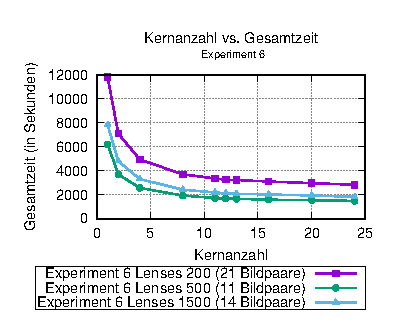
\includegraphics[width=\textwidth]{pdf/times_exp6}
			\caption[Experiment 6]{Experiment 6}
			\label{fig:times_exp6}
		\end{subfigure}
		\hfill
		\begin{subfigure}[b]{0.49\textwidth}
			\centering
			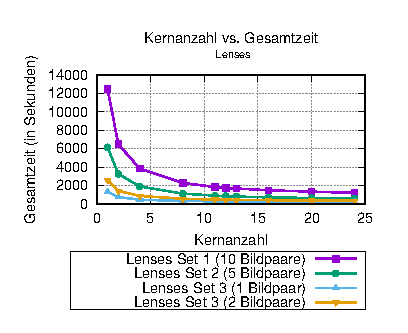
\includegraphics[width=\textwidth]{pdf/times_lenses}
			\caption[Lenses]{Lenses}
			\label{fig:times_lenses}
		\end{subfigure}
		\caption{Gesamtlaufzeiten}
		\label{fig:gesamtlaufzeiten}
	\end{figure}
\end{center}

Der Speedup des Programmes skaliert mit der Anzahl der Prozessorkerne nicht linear und flacht schnell ab. Der Speedup-Faktor für den \textit{Experiment 6} Datensätze übersteigt fünf nicht. Bei den \textit{Lenses}-Da\-ten\-sä\-tzen hingegen wird bei 24 Kernen ein Speedup von mehr als zehn erreicht. In den auf Abbildung \ref{fig:speedup} visualisierten Graphen ist eine starke Skalierung deutlich erkennbar. 

\begin{center}
	\begin{figure}
		\begin{subfigure}[b]{0.49\textwidth}
			\centering
			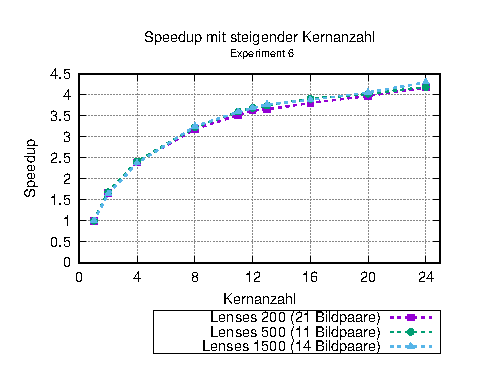
\includegraphics[width=\textwidth]{pdf/speedup_exp6}
			\caption[Experiment 6]{Experiment 6}
			\label{fig:speedup_exp6}
		\end{subfigure}
		\hfill
		\begin{subfigure}[b]{0.49\textwidth}
			\centering
			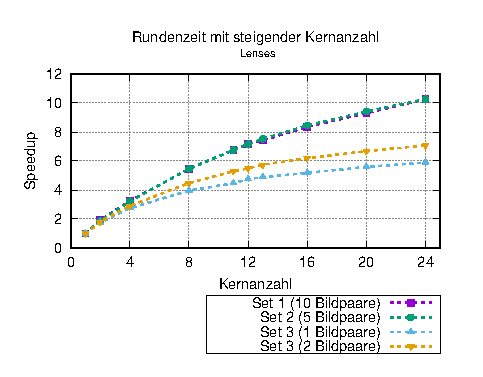
\includegraphics[width=\textwidth]{pdf/speedup_lenses}
			\caption[Lenses]{Lenses}
			\label{fig:speedup_lenses}
		\end{subfigure}
		\caption{Speedup}
		\label{fig:speedup}
	\end{figure}
\end{center}

Um Engpässe und besonders rechenaufwendige Funktionen zu identifizieren, wurde das Programm mit Zeitmessern versehen, die Ausführungszeiten und Aufrufanzahl protokolliert haben. Anschließend wurden es auf einem Rechenkern unter denselben Bedingungen, wie die anderen Konfigurationen, die Zeiten gemessen. Ein Überblick über das Gesamtprogramm mit seinen Subroutinen und deren Anteil an der Gesamtlaufzeit ist in Abbildung \ref{fig:perc_main} zu sehen.

\begin{center}
	\begin{figure}[htbp]
		\centering
		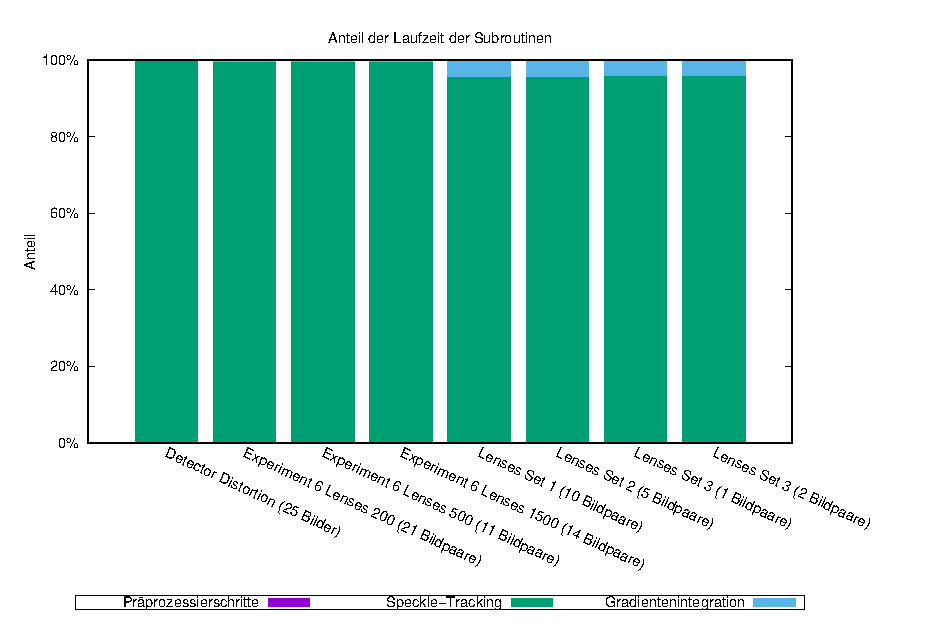
\includegraphics[width=0.7\textwidth]{pdf/main}
		\caption{Anteile der Laufzeiten}
		\label{fig:perc_main}
	\end{figure}
\end{center}

Hierbei ist eindeutig zu sehen, dass die meiste Zeit für das Speckle-Tracking benötigt wird. um weitere Informationen über die Laufzeiten der einzelnen Speckle-Tracking-Schritte zu gewinnen, wurde dieses ebenfalls mit Zeitmessern versehen. Die zeitliche Aufteilung dieser zeigt in Abbildung \ref{fig:perc_speckle}, dass hierbei der zweite Durchlauf am meisten Zeit benötigt. 

\begin{center}
	\begin{figure}[htbp]
		\centering
		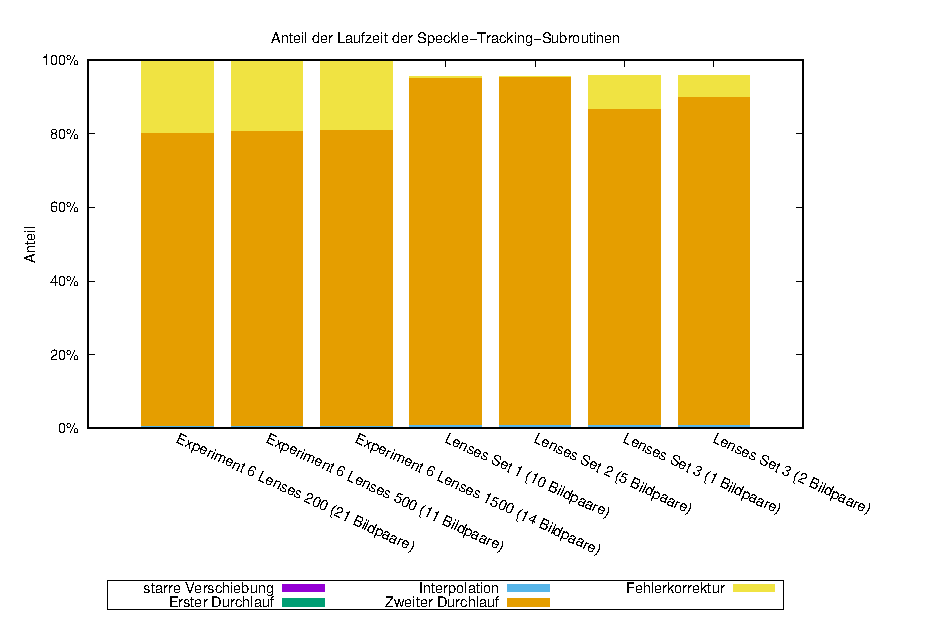
\includegraphics[width=0.7\textwidth]{pdf/speckle}
		\caption{Anteile der Laufzeiten des Speckle-Tracking-Algorithmus}
		\label{fig:perc_speckle}
	\end{figure}
\end{center}

Die kumulative Zeit der fünf rechenaufwendigsten Funktionen aller Konfigurationen, dargestellt in Abbildung \ref{fig:perc_slow}, liegt jeweils bei über 95\% der Gesamtzeit. 

\begin{center}
	\begin{figure}[htbp]
		\centering
		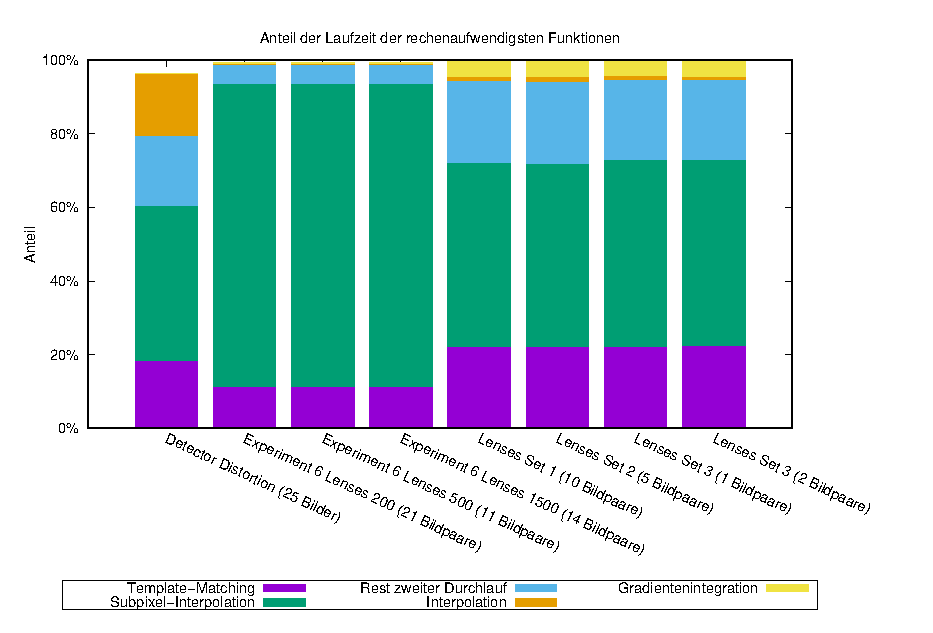
\includegraphics[width=0.7\textwidth]{pdf/slow}
		\caption{Anteile der Laufzeiten der langsamsten Funktionen}
		\label{fig:perc_slow}
	\end{figure}
\end{center}

\section{Grund der Performance-Engpässe}

Der Grund der langen Rechenzeiten des Template-Matchings und der Subpixel-Interpolation liegt in der hohen Anzahl der Aufrufe dieser begründet. Der zweite Durchlauf allein wird im \textit{Experiment 6 Lenses 200}-Datensatz über 5.3 Millionen mal aufgerufen. In jedem dieser Aufrufe wird das Template-Matching und die Subpixel-Interpolation jeweils ein mal genutzt. Hinzu kommt, dass, bis auf das Temp\-late-Match\-ing, der zweite Durchlauf nur geringen Gebrauch von bereits optimierten Bibliotheken wie numpy macht und somit der Pyhton-Overhead hinzukommt. 

Innerhalb des Speckle-Trackings ist der Aufruf des zweiten Durchlaufes mittels der joblib parallelisiert. Diese nutzt standardmäßig die multiprocessing-Bibliothek, welche für jeden Thread einen Fork der gesamten Python-Umgebung erstellen muss, was zu einem erheblichen Overhead führt\footnote{\url{https://pythonhosted.org/joblib/parallel.html}}.

Die hohe Rechenzeit der Gradienten-Integration ist im Aufruf dieser auf die Größe des Gesamtbildes begründet.

Insgesamt hat das Programm eine schlechte CPU-Auslastung von lediglich durchschnittlich 19,635\% \footnote{\url{https://github.com/ComputationalRadiationPhysics/Wavefront-Sensor/blob/f2fc5c2e5f8b4ef0e9b3ca3a4e770db67f230588/doc/cpu_util.md}}, wodurch häufig einige Kerne nicht oder nur wenig genutzt werden. 